\documentclass{beamer}

\setcounter{tocdepth}{1}

\mode<presentation> {
\usetheme{Antibes}
\definecolor{zelena}{rgb}{.9,.74,.00}
\usecolortheme[named=zelena]{structure}
}

\usepackage[T1]{fontenc}

\usepackage{hyperref} 
\usepackage{graphicx}
\usepackage{color}
\usepackage[english,serbian]{babel}
\usepackage[utf8]{inputenc}
\usepackage{listings}


\def\d{{\fontencoding{T1}\selectfont\dj}}
\def\D{{\fontencoding{T1}\selectfont\DJ}}

\title[Prepoznavanje saobraćajnih znakova pomoću CNN]{Prepoznavanje saobraćajnih znakova pomoću CNN}

\author{Jana Jovičić, Jovana Pejkić}
\institute[Matematički fakultet]
{
\small{Prezentacija seminarskog rada \\u okviru kursa\\ Računarska inteligencija \\ Matematički fakultet\\}
\medskip
\textit{jana.jovicic755@gmail.com, jov4ana@gmail.com}
}
\date{}

\begin{document}


\begin{frame}
\titlepage
\end{frame}

%------------------------------------------------


\begin{frame}
\frametitle{Sadržaj}
\tableofcontents
\end{frame}

%------------------------------------------------



\section{Cilj rada}
\begin{frame} 
\frametitle{Cilj rada}

\begin{itemize}
\item Za bazu podataka kineskih saobracajnih znakova izvršiti što precizniju klasifikaciju
\item Implementirati CNN u programskom jeziku Python uz korišćenje Keras biblioteke
\item Isprobati nekoliko različitih arhitektura mreže
\item Uporediti dobijene rezultate i izvesti zakljlučke
\end{itemize}


%\begin{figure}
%\includegraphics[width=270pt, height=126pt]{ime_slike.jpg}
%\caption{Naslov slike}
%\end{figure}

\end{frame}

%------------------------------------------------

\section{Informacije o korišćenom skupu podataka}
\begin{frame}
\frametitle{Informacije o korišćenom skupu podataka}

\begin{itemize}
\item Baza sadrži \textbf{6164 slika} saobraćajnih znakova
\begin{itemize}
\item podeljenih u \textbf{58 klasa}
\item pri čemu \textbf{trening skup} sadrži \textbf{4170 slika}
\item a \textbf{test skup 1994 slika}
\end{itemize}
\item Zbog nejednakog broja slika (negde 5, negde 400) po klasama, korišćen je deo baze
\item Izdvojeno je \textbf{10 klasa} koje su imale priblizno jednak broj slika
\item Dobijen je \textbf{trening skup} od \textbf{1693 slika} i \textbf{test skup} od \textbf{764 slika}


% TODO TODO TODO TODO TODO
% Na slici 10 je prikazan po jedan znak iz svake klase trening skupa, zajedno sa brojem elemenata te klase.
% Podaci o test skupu, mogu se videti na slici.
% Ubaciti slike pa srediti ovo zakomentarisano!

\end{itemize}

\end{frame}


%------------------------------------------------

%------------------------------------------------


\subsection{Unutrašnja struktura CNN}
\begin{frame}
\frametitle{Unutrašnja struktura CNN}

\begin{itemize}
\item \textbf{Konvolutivni sloj}
\begin{itemize}
\item Operacija konvolucije: $$(f * g)_{ij} = \sum_{k=0}^{p-1} \sum_{l=0}^{q-1} f_{i-k, i-l}*g_{k, l}$$
\end{itemize}
\item \textbf{Sloj agregacije}
\begin{itemize}
\item Maxpooling / Averagepooling
\end{itemize}
\item \textbf{Potpuno povezani sloj}
\begin{itemize}
\item Softmax funkcija
\item Categorical crossentropy
\end{itemize}
\end{itemize}

\begin{figure}
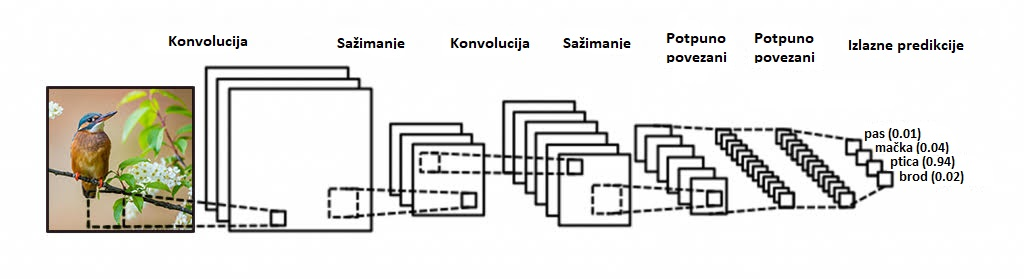
\includegraphics[scale=0.5]{cnn_layers.jpg}
\caption{Struktura konvolutivne neuronske mreže}
\end{figure}

\end{frame}



\subsection{Filtriranje i proširivanje}
\begin{frame}
\frametitle{Filtriranje, proširivanje i korak}

\begin{itemize}
\item Vrše se na konvolutivnom sloju
\item \textbf{Filtriranje} je ,,ekstraktovanje" karakteristika ulaza (slike)
\begin{itemize}
\item tako što se izvršava operacija konvolucije
\end{itemize}
\item Dimenzija mape nakon filtriranja je manja od dimenzije ulaza
\item Vrši se \textbf{proširivanje} ulazne matrice
\begin{itemize}
\item nulama / vrednostima koje su već na obodu
\end{itemize}
\item \textbf{Korak} - za koliko piksela se filter pomera duž slike
\end{itemize}

\begin{figure}
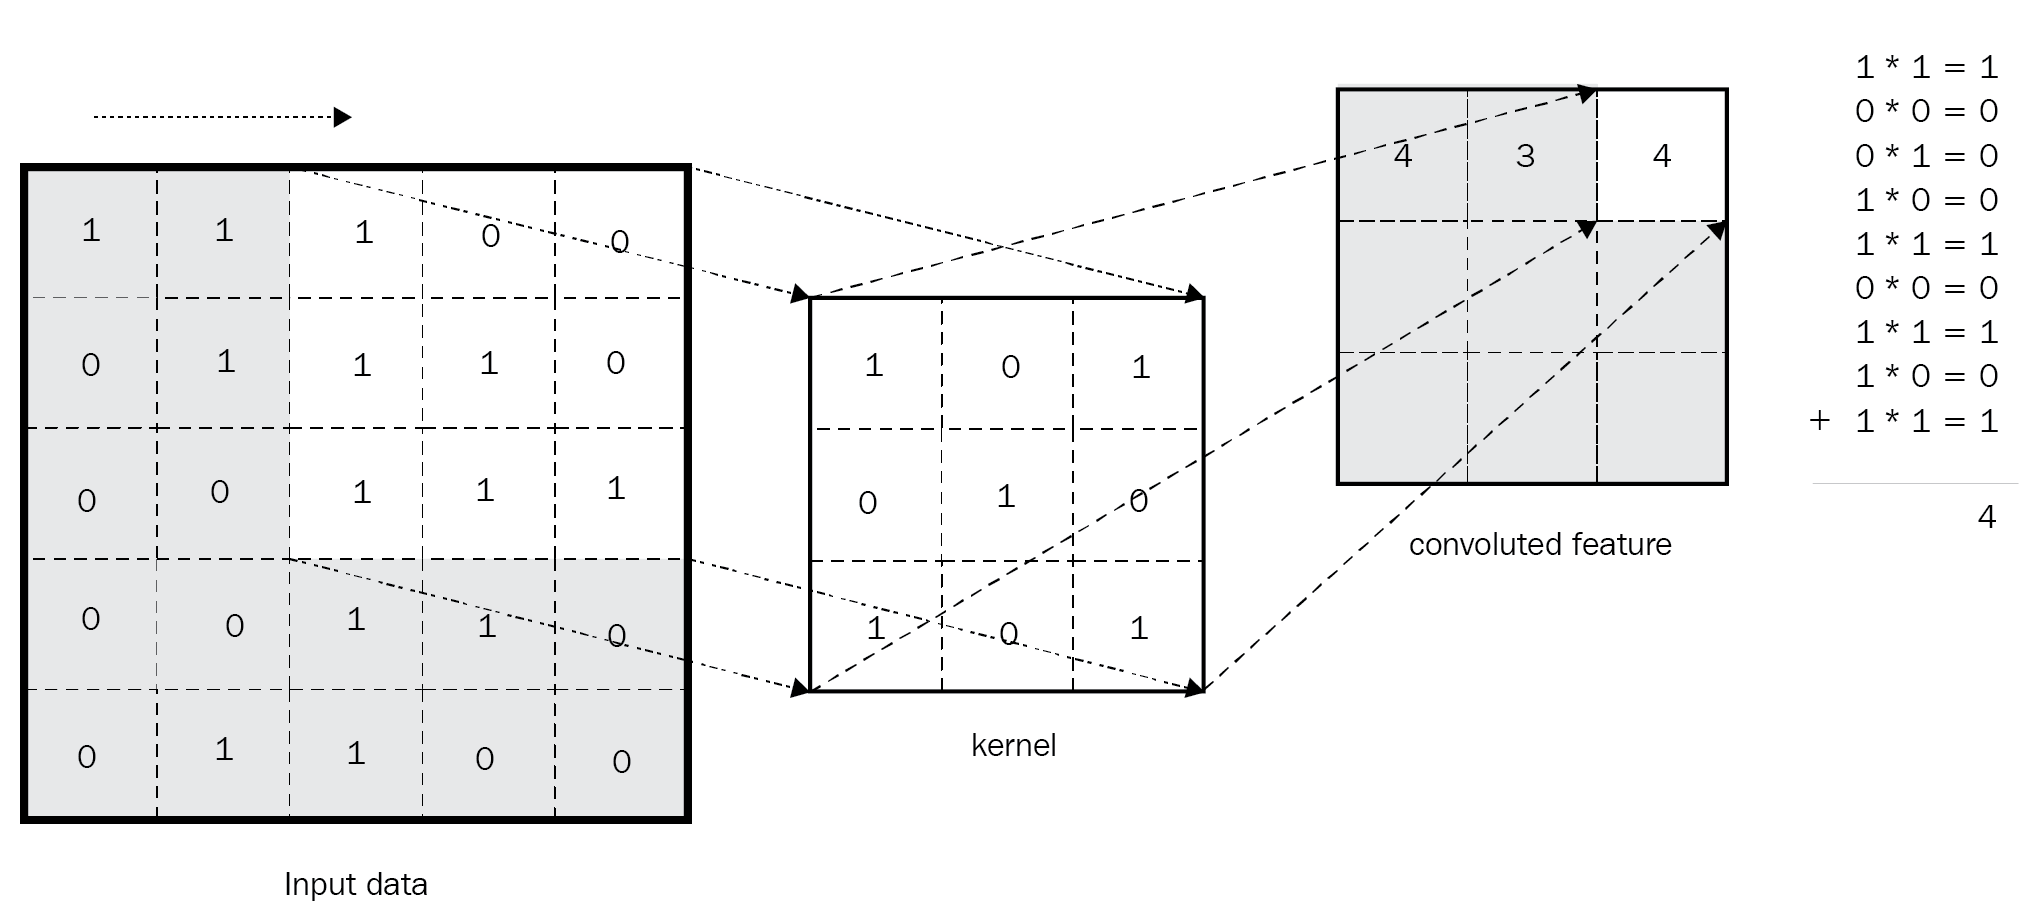
\includegraphics[scale=0.5]{filtriranje_mape.png}
\caption{Filtriranje}
\end{figure}


%\begin{Primer proširivanja ulazne matrice nulama}
%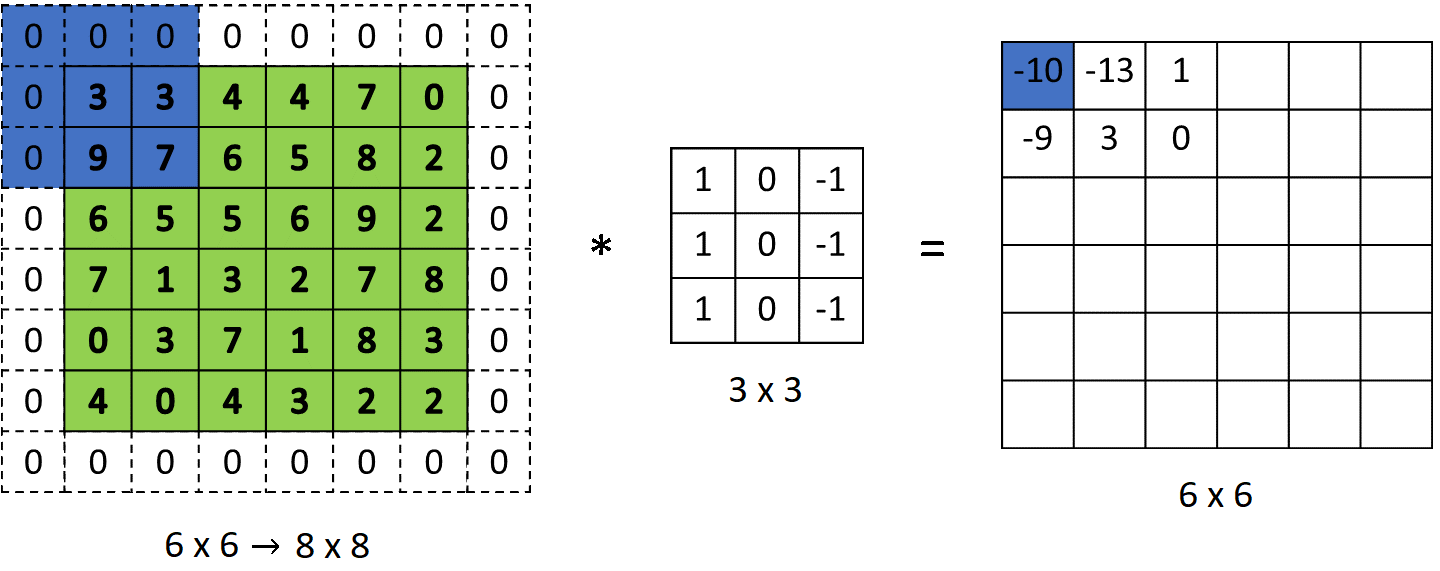
\includegraphics[scale=0.3]{padding.png}
%\caption{Primer proširivanja ulazne matrice nulama}
%\end{figure}

\end{frame}



\subsection{Aktivaciona funkcija}
\begin{frame}
\frametitle{Aktivaciona funkcija}

\begin{itemize}
\item Funkcija kojom se ograničavaju vrednosti izlaza neurona
\begin{itemize}
\item opseg izlaza neurona obično je u intervalu [0,1] ili [-1,1] \\
(osim za ReLU)
\end{itemize}
\item Više vrsta aktivacionih funkcija:
\begin{itemize}
\item \textbf{ReLU} (Rectified Linear Unit): $f(z)=max(0, z)$
\item \textbf{tanh}: $\tanh(x) = \dfrac{e^{2x}-1}{e^{2x}+1}$
\item \textbf{sigmoid}: $\sigma(x) = \dfrac{1}{1 + e^{-x}}$
\end{itemize}
\end{itemize}

%\begin{figure}
%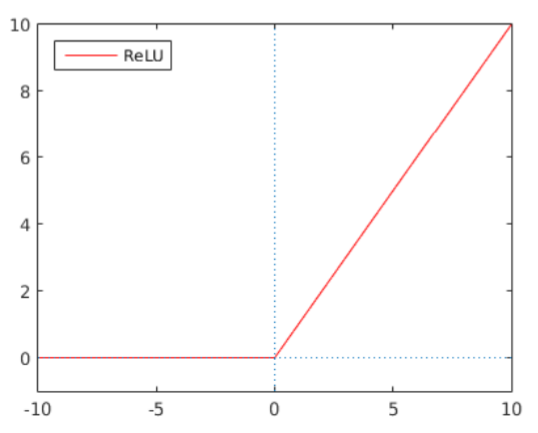
\includegraphics[scale=0]{relu_graph.png}
%\caption{Izgled ReLU funkcije}
%\end{figure}

\begin{figure}
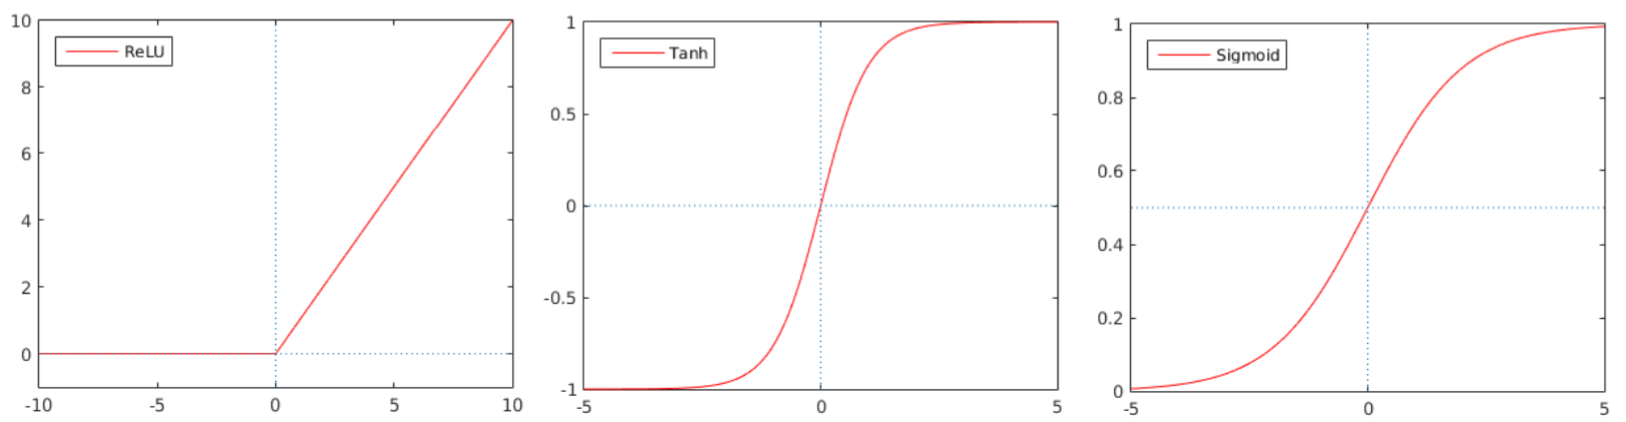
\includegraphics[scale=0.38]{graphs_prez.png}
\caption{Grafici funkcija: ReLU, tanh i sigmoid}
\end{figure}

\end{frame}


\subsection{Agregacija metodom Maxpool}
\begin{frame}
\frametitle{Agregacija metodom Maxpool}

\begin{itemize}
\item Jedan od metoda koji se koristi na sloju za agregaciju, najzastupljeniji
\item Vraća \textbf{maksimum} dela slike prekrivene filterom 
\item Ideja je da se informacije o slici što više ,,ukrupne"
\end{itemize}

\begin{figure}
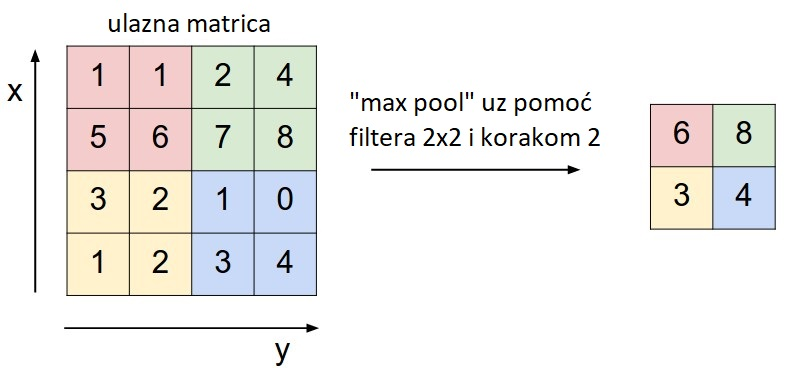
\includegraphics[scale=0.5]{maxpool.jpeg}
\caption{Metod Maxpool sa filterom [2x2] i korakom veličine 2}
\end{figure}

\end{frame}



\subsection{Potpuno povezani sloj}
\begin{frame}
\frametitle{Potpuno povezani sloj}

\begin{itemize}
\item Svaki neuron je povezan sa svakim neuronom iz prethodnog sloja
\item Kao ulaz očekuje vektor, što znači da je prvo potrebno ispraviti mapu karakteristika u vektor
\item Poslednji potpuno povezani sloj treba da ima onoliko neurona koliko ima i klasa
\item Poslednji sloj određuje koju klasu da pridruži slici pomoću softmax aktivacione funkcije
\item Softmax funkcija odreduje verovatnoću pripadnosti slike svakoj od klasa
\item Slika se klasifikuje u onu klasu kojoj odgovara najveća verovatnoća pripadnosti
\end{itemize}

\end{frame}


% -------------------
\begin{frame}
\frametitle{Potpuno povezani sloj - Funkcija gubitka}

\begin{itemize}
\item Funkcija gubitka: categorical crossentropy
\item Uporeduje raspodelu verovatnoća predvidenih klasa sa raspodelom koja odgovara pravim klasama
\item $$ H(y, \hat{y}) = -\sum_{i} y_i\cdot log(\hat{y})) $$
\item Služi da kvantifikuje kvalitet klasifikacije, tj. da oceni koliko je dobar skup težina koji služi za učenje mreže
\end{itemize}

\end{frame}

%------------------------------------------------

\subsection{Optimizacija mreže}
\begin{frame}
\frametitle{Optimizacija mreže}

\begin{itemize}
\item Cilj optimizacije: pronaći skup težina tako da se funkcija gubitka minimizuje
\item SGD (Stohastički Gradijentni Spust)
\begin{itemize}
	\item Težine se traže u pravcu koji je suprotan pravcu gradijenta funkcije gubitka - tako se može stići do lokalnog minimuma 
	\item Potrebno odrediti pogodnu dužinu koraka, tj. pronaći najbolji parametar učenja (learning rate)
	\item Ažuriranje težina moguće na osnovu samo dela podataka iz trening skupa
	\item Stohastički - nasumično bira trening uzorke na osnovu kojih će ažurirati parametre
	\item Održava jednu vrednost parametra učenja za sva ažuriranja težina i ta vrednost se
ne menja tokom treninga
\end{itemize}
\item Adam
\begin{itemize}
	\item Unapređena verzija SGD-a
	\item Može da održava različite parametre učenja za različite težine i da ih menja tokom procesa učenja
\end{itemize}
\end{itemize}

\end{frame}


%------------------------------------------------
%------------------------------------------------
%------------------------------------------------
%------------------------------------------------

\section{Modeli}

\subsection{Model 1}
\begin{frame}
\frametitle{Model 1}

\begin{itemize}

\item Jedan od prvih modela koji je imao uspeha nad test podacima
\item Sastoji se iz:
\begin{itemize}
\item 4 konvolutivna sloja
\item 2 agregirajuca sloja
\item 2 potpuno povezana sloja
\end{itemize}

\item U svim konvolutivnim slojevima:
\begin{itemize}
\item velicina jezgra je 3x3
\item broj filtera u konvolutivnom sloju je 32
\end{itemize}

% TODO TODO TODO TODO TODO Proveriti da li u svakom sloju?
% TODO TODO TODO TODO TODO Sta u svakom?

\item U svakom sloju se koristi \textbf{ReLU} aktivaciona funkcija
\item Agregacija se vrsi biranjem \textbf{maksimalne vrednosti} dela mape karakteristika koji je prekriven lterom

\end{itemize}


\end{frame}


\subsection{Model 1 nastavak}
\begin{frame}
\frametitle{Model 1 nastavak}

\begin{itemize}

\item Funkcijom \textbf{Dropout()} je isključivan određen broj nasumično odabranih neurona (da bi se sprečilo preprilagodjavanje)
\item Nakon agregacija je iskljuceno 20\% neurona, pre FC sloja 50\%

\item Poslednji potpuno povezani (FC) sloj
\begin{itemize}
\item ima onoliko neurona koliko ima klasa
\item koristi softmax aktivacionu funkciju
\end{itemize}

\item Ucenje modela je sprovedeno u 30 epoha
\item Batch size je postavljen na 32
\begin{itemize}
\item sto znaci da u svakoj iteraciji uzima 32 primerka iz trening skupa koja ce biti propagirana kroz mrezu
\end{itemize}

\item Optimizacija modela je izvrsena pomocu \textbf{SGD}
\item Sa tako podesenim parametrima preciznost je 0.88

\end{itemize}

\end{frame}

% --------------------

\subsection{Model 2: LeNet5}
\begin{frame}
\frametitle{Model 2: LeNet5}

\begin{itemize}
\item 7 slojeva: 2 konvolutivna, 2 average pooling, 3 potpuno povezana
\item Prvi konvolutivni sloj: 6 filtera veličine 3x3
\item Drugi konvolutivni sloj: 16 filtera veličine 3x3
\item ReLU aktivaciona funkcija
\item Potpuno povezani slojevi - broj neurona redom: 120, 84, koliko ima i klasa 
\item Pre treninga su slike skalirane na 32x32
\item Optimizacija pomoću Adam optimizatora
\item Prilikom učenja u 30 epoha sa batch size 32, preciznost je bila 0.91
\end{itemize}


\end{frame}

%------------------------------------------------


\subsection{Model 2 - nastavak}
\begin{frame}
\frametitle{Model 2 - nastavak}

\begin{figure}
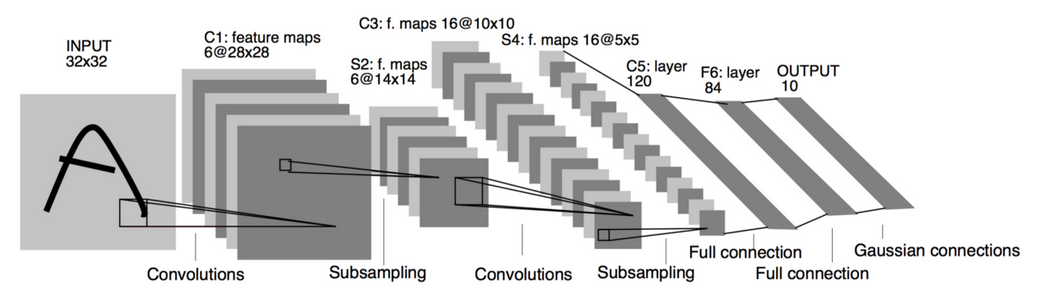
\includegraphics[scale=0.30]{lenet5_prez.png}
\caption{LeNet5 arhitektura}
\end{figure}

\end{frame}


% -------------------------------------

\subsection{Modeli 1 - statistike}
\begin{frame}
\frametitle{Modeli 1 - statistike}

\begin{figure}
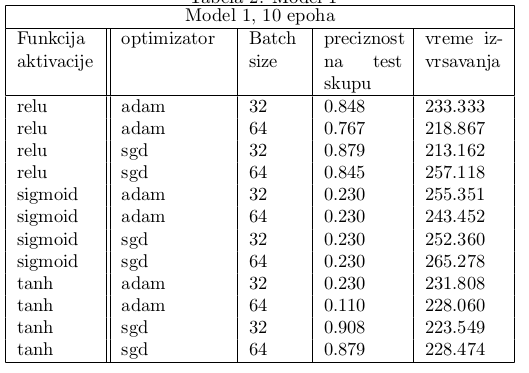
\includegraphics[scale=0.40]{stat_model1_10.png}
\caption{Rezultati Modela 1 za 10 epoha, različite vrednosti funkcije aktivacije (relu, tanh i sigmoid), optimizatora (SGD, Adam) i Batch size (32, 64)}
\end{figure}


\end{frame}

%------------------------------------------------

\subsection{Modeli 2 - statistike}
\begin{frame}
\frametitle{Modeli 2 - statistike}

\begin{figure}
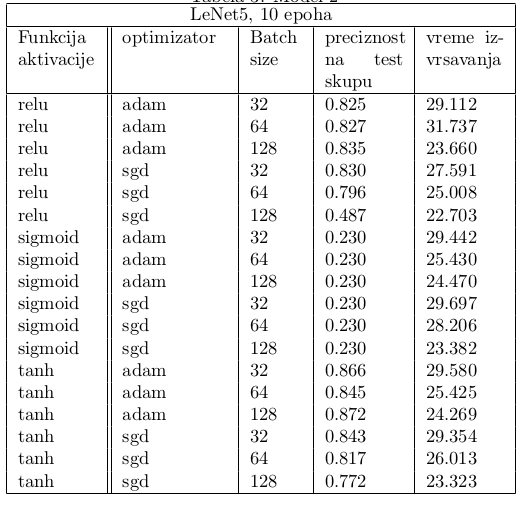
\includegraphics[scale=0.30]{stat_model2_10.png}
\caption{Rezultati LeNet5 modela za 10 epoha, različite vrednosti funkcije aktivacije (relu, tanh i sigmoid), optimizatora (SGD, Adam) i Batch size (32, 64 i 128)}
\end{figure}


\end{frame}

%------------------------------------------------

\subsection{Modeli 2 - statistike (nastavak)}
\begin{frame}
\frametitle{Modeli 2 - statistike (nastavak)}

\begin{figure}
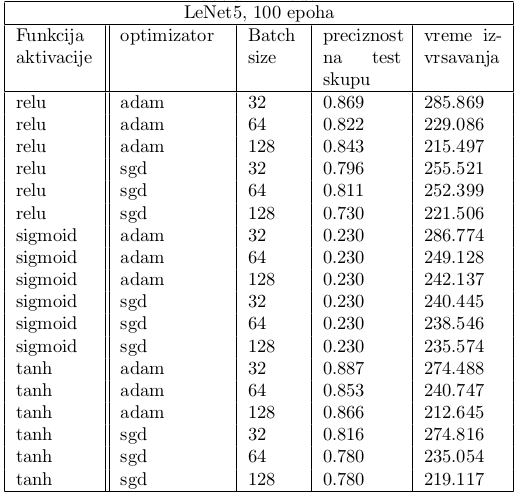
\includegraphics[scale=0.30]{stat_model2_100.png}
\caption{Rezultati LeNet5 modela za 100 epoha, različite vrednosti funkcije aktivacije (relu, tanh i sigmoid), optimizatora (SGD, Adam) i Batch size (32, 64 i 128)}
\end{figure}


\end{frame}

%------------------------------------------------

\subsection{Modeli 1 i 2 - poređenje}
\begin{frame}
\frametitle{Modeli 1 i 2 - poređenje}

\begin{itemize}
\item Sigmoidnu funkciju ne treba koristiti ni u modelu 1 ni u LeNet modelu, jer sve slike klasifikuje u istu klasu (8. klasu)
\item LeNet model je mnogo brži od modela 1: za približno isto vreme u modelu 1 se izvrsi 10 epoha, a u LeNet modelu 100 epoha
\item Kada se posmatra izvrsavanje u 10 epoha, model 1 daje malo bolje rezultate od LeNet (ako se izuzme kombinacija tangentne aktivacione funkcije i optimizacije pomocu Adama)
\item Model 1 daje najveću preciznost (0.908) na test skupu u 10 epoha kada se kao aktivaciona funkcija koristi tangenta funkcija, kada se optimizuje pomoću SGD i kada je batch size = 32
\end{itemize}

\end{frame}

%------------------------------------------------

\subsection{Modeli 1 i 2 - poređenje (nastavak)}
\begin{frame}
\frametitle{Modeli 1 i 2 - poređenje (nastavak)}

\begin{itemize}
\item Model 1 ima nesto veću preciznost kada je batch size = 32, u odnosu na to kada je batch size = 64
\item Kada poredimo izvršavanje LeNet modela u 10 i 100 epoha, vidimo da je preciznost tek malo bolja u 100 epoha, nego u 10 - za 0.01 ili 0.02. A izvrsavanje traje oko 10 puta duže. Zato se više isplati uzeti manji broj epoha.
\end{itemize}

\end{frame}

%------------------------------------------------
%------------------------------------------------
%------------------------------------------------
%------------------------------------------------



\subsection{Model 3: AlexNet}
\begin{frame}
\frametitle{Model 3: AlexNet}

\begin{itemize}
\item AlexNet arhitektura je jedna od prvih dubokih mreža
\item Sastoji se iz:
\begin{itemize}
\item 5 konvolutivna sloja
\item 3 potpuno povezana sloja
\end{itemize}
\item Kao aktivaciona funkcija koristi se ReLu
\end{itemize}


\begin{figure}
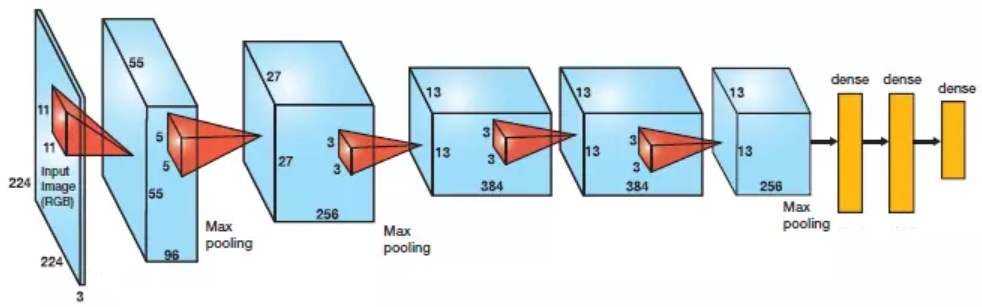
\includegraphics[scale=0.55]{alexnet_arh.png}
\caption{AlexNet arhitektura}
\end{figure}


\end{frame}



\subsection{Model 3: AlexNet - nastavak}
\begin{frame}
\frametitle{Model 3: AlexNet - nastavak}

\begin{itemize}
\item Mreža koju smo implementirale svaki izlaz iz konvolutivnog sloja normalizuje pre nego što ga prosledi narednom sloju
\item Pre normalizacije (nakon 1., 2. i 5. konv. sloja) - agregacija
\begin{itemize}
\item sa parametrom padding = 'valid' (nema proširenja)
\end{itemize}
\item Poravnavajući sloj ("ispravlja" mapu karakteristika u vektor)
\item 3 Dense sloja + Dropout()
\begin{itemize}
\item Dropout() sprečava preprilagodavanje modela
\end{itemize}
\item Na kraju je izlazni sloj koji preslikava ulaz u zadati broj klasa
\begin{itemize}
\item kao funkciju aktivacije koristi Softmax.
\end{itemize}
\end{itemize}

%\begin{figure}
%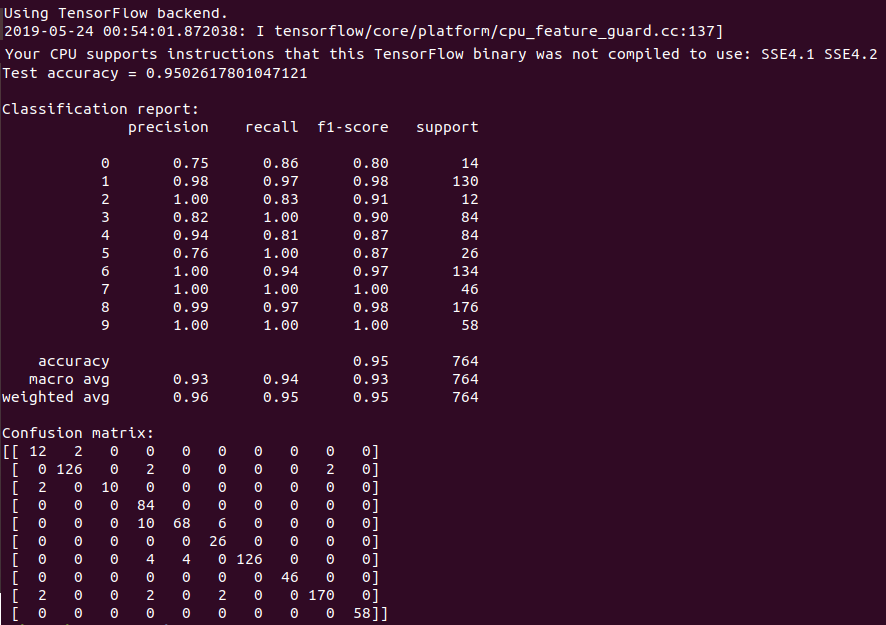
\includegraphics[scale=0.5]{confussion_matrix_alexNet_1000epoh.png}
%\caption{Matrica konfuzije i ostale statistike AlexNet modela za 1000 epoha}
%\end{figure}

\end{frame}


\subsection{Model 3: AlexNet - statistike}
\begin{frame}
\frametitle{Model 3: AlexNet - statistike}

\begin{itemize}
\item Kod AlexNet modela, vreme izvršavanja je oko 10 puta veće za 100 nego za 10 epoha

\item Najmanja preciznost za AlexNet model se postiže za funkciju sigmoid, 10 epoha i Batch size 256, a iznosi 0.696

\begin{itemize}
\item to je jedini slučaj da je preciznost ispod 0.71
\item uglavnom su preciznosti u intervalu [0.801, 0.934]
\item ne osciluje mnogo izvan pomenutog intervala
\end{itemize}

\item Prosečna preciznost za 10 epoha je 82\%, a za 100 epoha 90\%

\item Iz ovoga se može zaključiti da je za AlexNet model i dati skup podataka
bolje trenirati model u što više epoha
\item Ovo potvrduje i činjenica da je u 1000 epoha ovaj model dostigao najveću preciznost od 95\% (veću od sva tri modela)

\end{itemize}

\end{frame}


\subsection{Model 3: AlexNet - statistike - nastavak}
\begin{frame}
\frametitle{Model 3: AlexNet - statistike - nastavak}

\begin{figure}
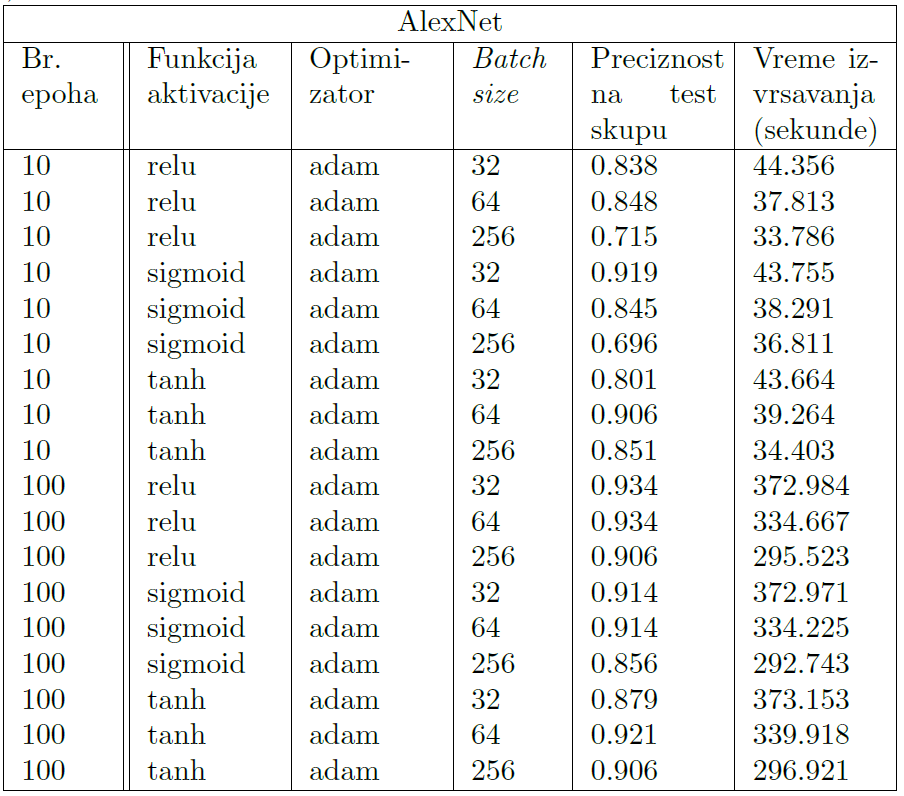
\includegraphics[scale=0.42]{alexNet_tabela.png}
\caption{Rezultati za AlexNet model za različite vrednosti broja epoha (10 i 100), funkcije aktivacije (relu, tanh i sigmoid) i Batch size (32, 64 i 256)}
\end{figure}

\end{frame}



\subsection{AlexNet i LeNet-5}
\begin{frame}
\frametitle{AlexNet i LeNet-5}

\begin{itemize}
\item Primetiti da se vrednosti na y-osi ova dva grafika razlikuju
\item To je zato što LeNet-5 daje malu preciznost za f-ju sigmoid
\item U 100 epoha maksimalna preciznost AlexNet mreže je 0.934, a LeNet-5 0.887

\end{itemize}

\begin{figure}
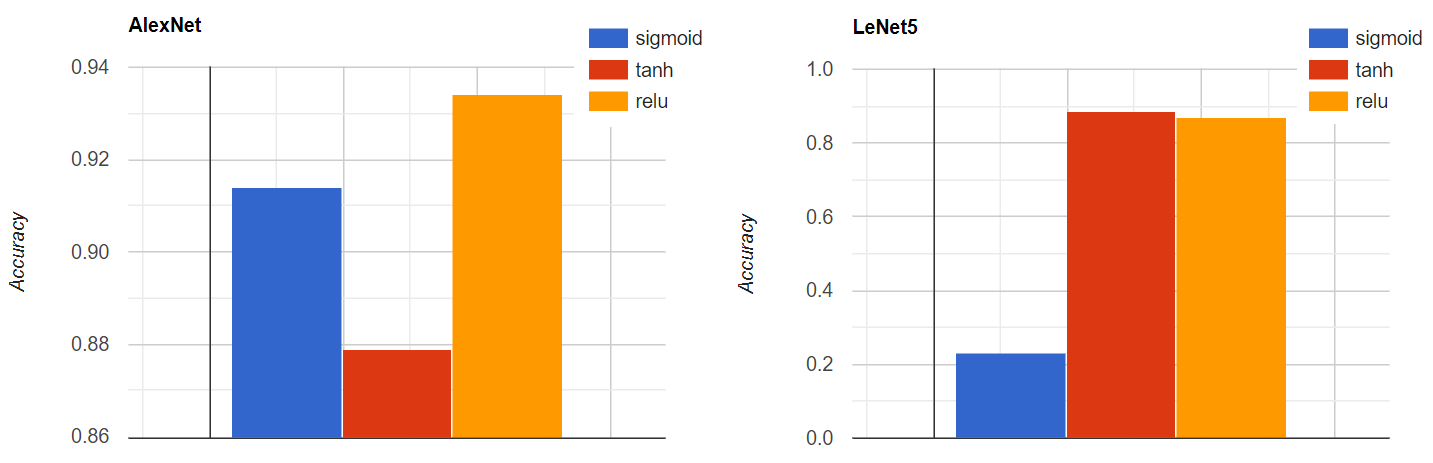
\includegraphics[scale=0.45]{graphs_alexnet_lenet.png}
\caption{Grački prikaz preciznosti za mreže AlexNet i LeNet-5 za 100 epoha, za funkcije sigmoid, tanh i ReLu}
\end{figure}

\end{frame}


%------------------------------------------------

%------------------------------------------------





\section{Zaključak}

\begin{frame}
\frametitle{Zaključak}

\begin{itemize}
\item Za sva tri isprobana modela mreža moguće je naći parametre tako da dobro klasifikuju test podatke 
\item Od svega što smo probale, najbolje rezultate (preciznost od 0.95) je dala AlexNet mreža u 1000 epoha
\end{itemize}

\end{frame}

%------------------------------------------------

\section{Literatura}

\begin{frame}
\frametitle{Literatura}
\footnotesize{
\begin{thebibliography}{99}

\bibitem[]{p1} Mladen Nikolić, Andelka Zečević
\newblock \small{\textbf{Mašinsko učenje}, 2019.}

\bibitem[]{p1} Saad Albawi
\newblock \small{\textbf{Understanding of a Convolutional Neural Network}, 2017.}

\bibitem[]{p1} Leon Bottou, Yann LeCun, Patric Haffner
\newblock \small{\textbf{Object recognition with Gradient-Based learning}, 1998. }

\end{thebibliography}
}

\end{frame}
%------------------------------------------------

%\begin{frame}
%\Huge{\centerline{Hvala na pažnji!}}
%\end{frame}


\end{document} 
